\documentclass[12pt]{amsart}
\usepackage{amssymb}
\usepackage{tikz}
\usepackage{color}

\begin{document}

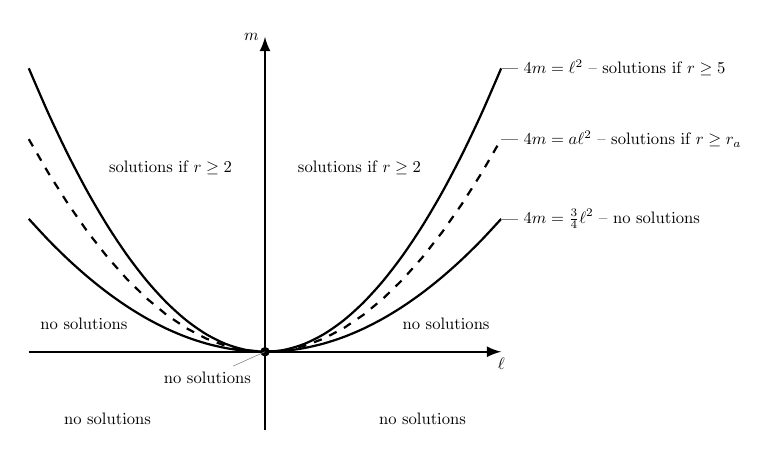
\begin{tikzpicture}
\draw[thick, -latex] (-3,0) -- (3,0) node[below,scale=0.6] {$\ell$};
\draw[thick, -latex] (0,-1) -- (0,4) node[left,scale=0.6] {$m$};

\draw[scale=1, domain=-3:3, smooth, variable=\x,  thick] plot ({\x}, {0.4*\x*\x});
\coordinate[pin={[pin distance=10,scale=0.6]0:$4m=\ell^2$ -- solutions if $r\geq 5$}] (r1) at (3,0.4*3*3);

\draw[scale=1, domain=-3:3, smooth, variable=\x,  thick] plot ({\x}, {0.1875*\x*\x});
\coordinate[pin={[pin distance=10,scale=0.6]0:$4m=\frac{3}{4}\ell^2$ -- no solutions}] (r1) at (3,0.1875*3*3);

\draw[scale=1, domain=-3:3, dashed, variable=\x,  thick] plot ({\x}, {0.3*\x*\x});
\coordinate[pin={[pin distance=10,scale=0.6]0:$4m=a \ell^2$ -- solutions if $r\geq r_a$}] (r1) at (3,0.3*3*3);

\node[below,scale=0.6] at (1.2,2.5) {solutions if $r\geq 2$};
\node[below,scale=0.6] at (-1.2,2.5) {solutions if $r\geq 2$};
\node[below,scale=0.6] at (2.3,0.5) {no solutions};
\node[below,scale=0.6] at (-2.3,0.5) {no solutions};
\node[below,scale=0.6] at (2.,-.7) {no solutions};
\node[below,scale=0.6] at (-2.,-.7) {no solutions};
\filldraw [black] (0,0) circle (1.5pt);
 \coordinate[pin={[pin distance=10,scale=0.6]240:no solutions}] (r1) at (0,0);
\end{tikzpicture}

\end{document}